\chapter{Ex 6}

\section{Geometrische Gestalt der Kerne}

\subsection{Mandelstam-Variablen}
Betrachten die Reaktion zweier Teilchen mit den 4-Impulsen $p_1$ und $p_2$. Die auslaufenden Teilchen sollen die 4-Impulse $p_3$ und $p_4$ haben.
Dann kann man die sogen. \textbf{Mandelstam-Variablen}
\begin{alignat*}{3}
	s &= \left(p_1 + p_2 \right)^2 &&= \left(p_3 + p_4 \right)^2 \\
	t &= \left(p_1 - p_3 \right)^2 &&= \left(p_4 - p_2 \right)^2 \\
	u &= \left(p_1 - p_4 \right)^2 &&= \left(p_3 - p_2 \right)^2.
\end{alignat*}
$s$ ist dabei das Quadrat der Schwerpunktsenergie des Systems und $u$ entspricht dem Quadrat des 4-Impulsübertrags einer gewöhnlichen Streuung.
Die Mandelstam-Variablen sind Lorentzskalare.

\subsection{Die Rapidität}
Die Rapidität ist ein Maß für Geschwindigkeiten in der Relativistik.
Sie ist definiert als
\begin{equation*}
	y = \frac{1}{2}\log\left(\frac{E+cp}{E-cp}\right)\quad \text{bzw. als}\quad y_L=\frac{1}{2}\log\left(\frac{E+cp_\text{z}}{E-cp_\text{z}}\right)
\end{equation*}
in der Teilchenphysik.
Anders als die Geschwindigkeit $v$ eines Teilchens ist die Rapidität nicht auf das Intervalll $[-c,\ +c]$ beschränkt, sondern ist unbeschränkt.
Sie gibt ein intuitiveres Gefühl dafür, welche Geschwindigkeit ein Teilchen hätte, würde es keine relativistischen Effekte erfahren.
Außerdem sind Differenzen von zwei Rapiditäten invariant unter Lorentzboosts entlang der Strahlachse und man kann Rapiditäten einfach addieren, anders als Geschwindigkeiten ($\rightarrow$ rel. Geschwindigkeitsaddition).
Aufgrund dieser Invarianz unter Lorentzboosts wird die Angabe von $y$ gegenüber dem Polarwinkel $\theta$ bevorzugt.

Für den Fall $E\gg m$ geht die Rapidität über in die sogen. \textbf{Pseudorapidität}
\begin{equation*}
	\eta = -\log\left(\tan\left(\frac{\theta}{2}\right)\right).
\end{equation*}

Der diferenzielle Wirkungsquerschnitt $\nicefrac{\text{d}\sigma}{\text{d}y}$ ist forminvariant unter Lorentzboosts entlang der Strahlachse.
Das gleiche gilt in guter Näherung auch für $\nicefrac{\text{d}\sigma}{\text{d}\eta}$, allerdings ist $\eta$ einfacher zu messen, da man nur die Flugrichtung des Teilchens durch den Detektor bestimmen muss.

\subsection{Elastische Streuung punktförmiger Teilchen}
Streuexperimente dienen dazu, Mikroskopie über das sichtbare hinaus zu betreiben und so Erkenntnisse über die Struktur der Materie zu gewinnen.
Man unterscheidet dabei zwischen \textbf{elastischer} ($\sum E_{\text{kin,}i} = \sum E_{\text{kin,}f}$) und \textbf{inelastischer Streuung} ($\sum E_{\text{kin,}i} \neq \sum E_{\text{kin,}f}$, z.B. durch Anregung eines Atoms durch Teil der kinetischen Energie).

Der Wirkungsquerschnitt ist die wichtigste Größe bei solchen Experimenten und ist ein Maß dafür, wie wahrscheinlich eine Wechselwirkung zwischen dem Projektil und dem Target ist.
Experimentell gilt
\begin{equation*}
	\sigma = \frac{N_\text{obs}-N_\text{bg}}{\mathcal{L}\cdot\varepsilon\cdot A}\cdot\frac{1}{T},
\end{equation*}
mit der weiteren wichtigen Detektorkenngröße, der \textbf{Luminosität} $\mathcal{L}$.

\subsubsection{Rutherford-Wirkungsquerschnitt}
Der Rutherfordsche Wirkungsquerschnitt gibt den theoretischen Wirkungsquerschnitt unter Vernachlässigung von Spins und Targetrückstoß an
\begin{equation}\label{eq:ruth_sigma}
	\left(\diff[\sigma]{\Omega}\right)_\text{Ruth} = \left(\frac{zZe^2}{4\pi\epsilon_0\cdot 4E_\text{kin}}\right)^2\cdot\frac{1}{\sin^4\frac{\theta}{2}}.
\end{equation}

Definiert man den Impulsübertrag
\begin{equation*}
	\mvec{q} = \mvec{p}-\mvec{p'},
\end{equation*}
so lässt sich \autoref{eq:ruth_sigma} auch schreiben als
\begin{equation*}
	\left(\diff[\sigma]{\Omega}\right)_\text{Ruth} = \frac{4zZ\alpha^2(\hbar c)^2 E'^2}{|\mvec{q}c|^4}.
\end{equation*}
Durch die $\nicefrac{1}{q^4}$-Abhängigkeit ist es schwer, Prozesse mit hohem Impulsübertrag zu messen, da ein Fehler auf $\mvec{q}$ sich erheblich auf die Ergebnisse auswirkt.

Beachtet man, dass für kleine Massen $E\approx pc$ gilt, folgt daraus der \textbf{relativistische Rutherford-Wirkungsquerschnitt}
\begin{equation*}
	\left(\diff[\sigma]{\Omega}\right)_\text{Ruth} = \left(\frac{zZ\alpha\hbar c}{4mc^2(\gamma-1)}\right)^2\cdot\left(\frac{4p_1p_3}{q^2}\right)^2.
\end{equation*}

\subsubsection{Mott-Wirkungsquerschnitt}
Ist nun der Spin des Projektiles $\neq 0$, ergibt sich daraus der \textbf{Mott-Wirkungsquerschnitt}
\begin{equation*}
	\left(\diff[\sigma]{\Omega}\right)_\text{Mott} = \left(\diff[\sigma]{\Omega}\right)_\text{Ruth}\cdot\underbrace{\frac{E_\text{f}}{E}}_\text{Targetrückstoß}\cdot\underbrace{\left(1-\beta^2\sin^2\frac{\theta}{2}\right)}_\text{Spin d. Projektils}.
\end{equation*}
Für $\beta\rightarrow 1$ geht der Wirkungsquerschnitt über in
\begin{equation*}
	\left(\diff[\sigma]{\Omega}\right)_\text{Mott}= \rightarrow\left(\diff[\sigma]{\Omega}\right)_\text{Ruth}\cdot\frac{E_\text{f}}{E}\cdot\cos^2\frac{\theta}{2}.
\end{equation*}
Dabei sieht man, dass für $\beta\rightarrow 1$ ein Streuwinkel von 180° nicht möglich ist.
Dies folgt aus der Helizitätserhaltung: Bei einer Rückstreuung müsste auch der Spin flippen, damit die Projektion des Spins auf die Flugbahn (Helizität) erhalten bleibt. Dies ist jedoch an einem spinlosen Target aufgrund der Drehimpulserhaltung nicht möglich.

\subsubsection{Dirac-Wirkungsquerschnitt}
Bei der \textbf{Dirac-Streuung} haben nun beide Streupartner einen Spin.
Der Wirkungsquerschnitt wird dementsprechend modifiziert
\begin{equation*}
	\left(\diff[\sigma]{\Omega}\right)_\text{Dirac} = \left(\diff[\sigma]{\Omega}\right)_\text{Mott}\cdot\left(1+2\tau\tan^2\frac{\theta}{2}\right),
\end{equation*}
wobei $\tau = \frac{Q^2}{4M^2c^2}$.
Damit kann allerdings keine Streuung z.B. an realen Protonen beschrieben werden, da hier angenommen wird, dass das \textbf{punktförmige} ''Dirac-Proton'' ein herkömmliches magnetisches Moment von $\mu=\frac{e}{2m}$ besitzt.

\subsection{Elastische Streuung ausgedehnter Teilchen}

\begin{figure}
	\centering
	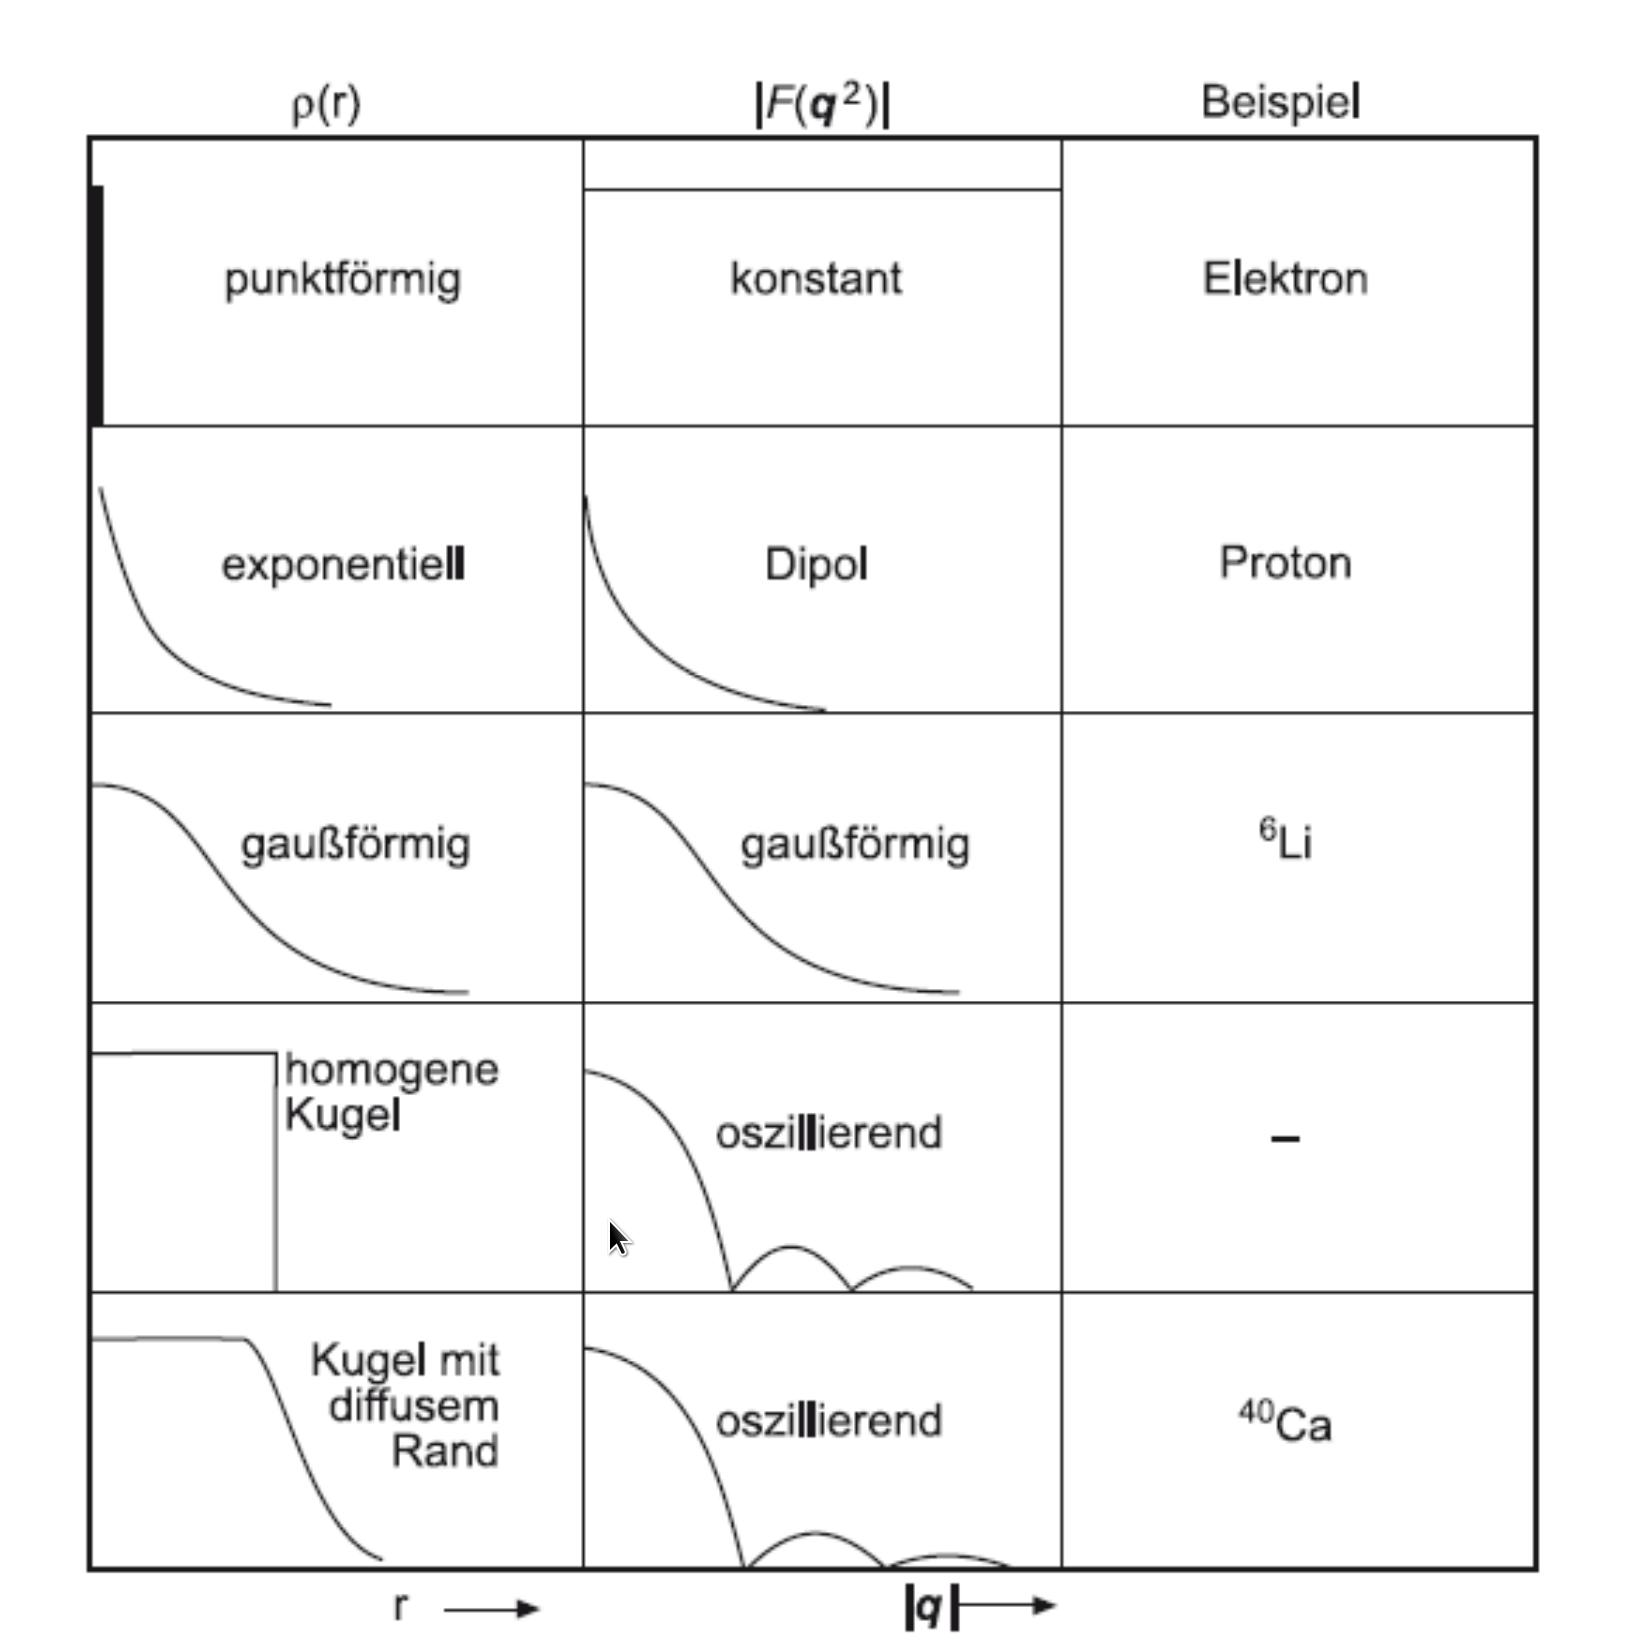
\includegraphics[width=.5\textwidth]{./img/formfaktoren_rho.jpeg}
	\caption{\textbf{Formfaktoren und zugehörige Ladungsverteilungen}}
	\label{fig:formfaktoren}
\end{figure}

\subsubsection{Formfaktoren}
In der Realität stellt man bei Streuexperimenten einen Unterschied zwischen dem theoretischen und gemessenen Mott-Wirkungsquerschnitt fest.
Dabei konvergieren die gemessenen Wirkungsquerschnitte nur für den Grenzfall verschwindender Impulsüberträge gegen den theoretischen Mott-Querschnitt und werden mit steigendem $|\mvec{q}|$ systematisch kleiner.
Der Grund hierfür ist, dass die Nukleonen und Kerne in Wirklichkeit ausgedehnte Objekte sind.
Somit ''sieht'' das Elektron bei der Streuung mit größerem $|\mvec{q}|$ nicht mehr die gesamte Ladung des Targets.
Der räumlichen Ausdehnung kann durch einen \textbf{Formfaktor $F(q^2)$} Rechnung getragen werden.
Da es bei kugelsymmetrischen Systemen keine Vorzugsrichtung gibt, hängt der Formfaktor dabei nur vom Betrag von $\mvec{q}$ ab.
Der Zusammenhang zwischen dem so angepassten Wirkungsquerschnitt und dem Mott-Wirkungsquerschnitt ist durch
\begin{equation*}
	\left(\diff[\sigma]{\Omega}\right)_\text{exp} = \left(\diff[\sigma]{\Omega}\right)_\text{exp}\cdot \left|F(q^2)\right|^2
\end{equation*}
gegeben.

Dabei kann in \textsc{Born}scher Näherung und unter Vernachlässigung des Targetrückstoßes der Formfaktor durch die Fouriertransformierte der Ladungsverteilung als
\begin{equation*}
	F(q^2) = \int{\text{d}^3x\ \rho(\mvec{x})e^{\frac{i}{\hbar}\mvec{q}\cdot\mvec{x}}}
\end{equation*}
ausgedrückt werden.

Theoretisch ließe sich durch inverse Fouriertransformation so Rückschluss auf die radiale Ladungsverteilung des Targets ziehen.
Dies ist in der Praxis jedoch nur beschränkt möglich, da der Wirkungsquerschnitt für steigende $|\mvec{q}|$ sehr schnell abnimmt und der Formfaktor generell nur über einen beschränkten Bereich bestimmt werden kann.
Dies resultiert daraus, dass der mögliche Impulsübertrag durch die Strahlenergie beschränkt ist.
Daher wählt man für gewöhnlich eine Parametrisierung von $\rho(r)$, bestimmt daraus den Formfaktor und variiert danach so lange die Parameter, bis die Modellfunktion mit den Messdaten übereinstimmt.
\autoref{fig:formfaktoren} zeigt Beispiele für verschiedene $\rho-F$ Paare.

\begin{figure}
	\centering
	\includegraphics[width=.5\textwidth]{./img/rosenbluth.pdf}
	\caption[Elektrischer und magnetischer Formfaktor von Proton und Neutron]{\textbf{Elektrischer und magnetischer Formfaktor von Proton und Neutron} aufgetragen gegen $Q^2$. Die Datenpunkte für $G_\text{M}^\text{n}$ und $G_\text{M}^\text{p}$ sind mit den angegebenen Faktoren skaliert und liegen dann übereinander}
	\label{fig:rosenbluth}
\end{figure}
Die Streuung eines Elektrons an einem Nukleon wird beispielsweise durch die \textbf{Rosenbluth-Formel}
\begin{equation*}
	\left(\diff[\sigma]{\Omega}\right)_\text{Rb} = \left(\diff[\sigma]{\Omega}\right)_\text{Mott}\cdot\left(\frac{G_\text{E}^2(Q^2) + \tau G_\text{M}^2(Q^2)}{1+\tau} + 2\tau\cdot G_\text{M}^2(Q^2)\tan^2\frac{\theta}{2}\right)
\end{equation*}
beschrieben. Es sind zwei Formfaktoren $G_\text{E}(Q^2)$ und $G_\text{M}(Q^2)$ nötig, um die elektrischen und magnetischen Verteilungen zu charakterisieren.
Sie hängen von $Q^2$ ab, daher kann man durch eine Messung der $Q^2$-Abhängigkeit auf die räumliche Verteilung von Ladung und magnetischem Moment schließen.
Im Grenzfall $Q^2\rightarrow 0$ entspricht dabei $G_\text{E}$ der auf die Elementarladung normierten elektrischen Ladung und $G_\text{M}$ dem auf das Kernmagneton normierten magnetischen Moment des Targets.
Man kann die Formfaktoren bestimmen, indem man den Wirkungsquerschnitt für jeweils feste Werte von $Q^2$ bei verschiedenen Streuwinkeln $\theta$ misst und durch den Mott-Querschnitt teilt.
Dann trägt man das Resultat gegen $\tan^2\frac{\theta}{2}$ auf, damit liegen die Messwerte auf einer Geraden, aus deren Achsabschnitt und Steigung sich die Formfaktoren bestimmen lassen.
\autoref{fig:rosenbluth} zeigt die Messung der Formfaktoren $G$ in Abhängigkeit des Impulsübertrages $Q^2$.
